\begin{figure}
    \centering
    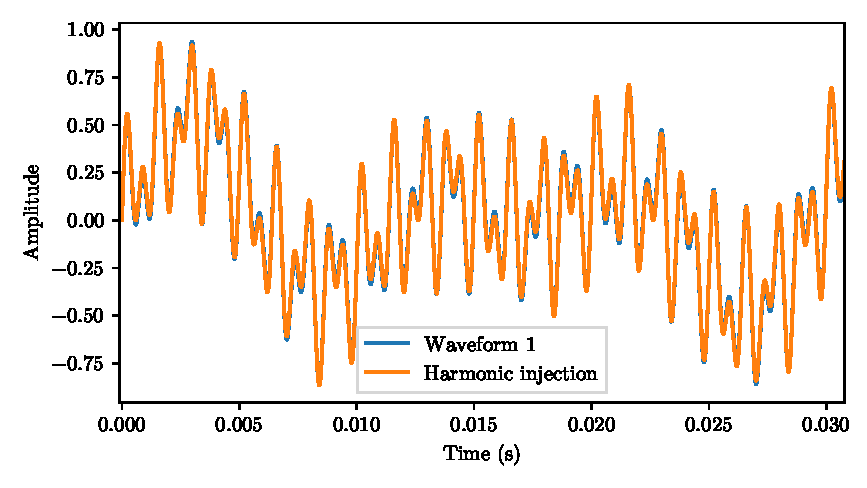
\includegraphics{Images/shaker/Figure_1.pdf}
    \caption{Waveform comparison of the shaker test.}
    \label{fig:shaker}
\end{figure}

\begin{figure}
    \centering
    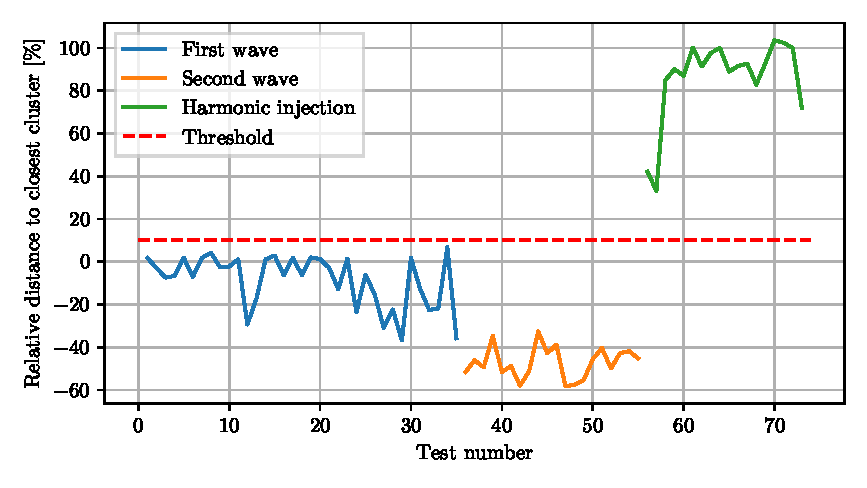
\includegraphics{Images/shaker/Results.pdf}
    \caption{Novelty detection result}
    \label{fig:shaker_results}
\end{figure}

\begin{figure}
    \centering
    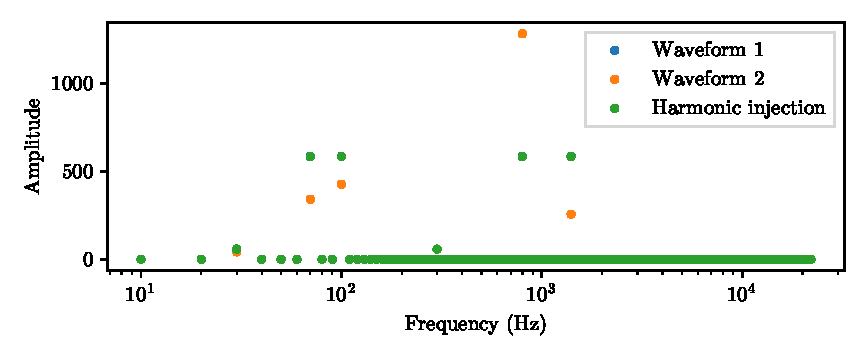
\includegraphics{Images/shaker/spectrum.pdf}
    \caption{Spectrum of the waveforms.}
    \label{fig:shaker_spectrum}
\end{figure}

\begin{table}
    \centering
    \caption{Harmonic coefficients for the shaker test. Wave 1 and Wave 2 are training signals, and Harmonic Injection is the signal to be detected.}
    \label{tab:shaker_param_01}
    \begin{tabular}{lccccccc} 
    \toprule
    \multirow{2}{*}{\textbf{Signal Name }} & \multicolumn{6}{c}{\textbf{Harmonic frequency} [Hz]} & \multirow{2}{*}{\textbf{Amplitude} [mV]$_{pp}$} \\
     & 30 & 70 & 100 & 300 & 800 & 1400 &  \\ 
    \hline
    Wave 1 & 0.1 & 1.0 & 1.0 & \multicolumn{1}{c}{-} & 1.0 & 1.0 & 1000 \\
    Wave 2 & 0.1 & 0.8 & 1.0 & \multicolumn{1}{c}{-} & 3.0 & 0.6 & 1000 \\
    Harmonic Injection & 0.1 & 1.0 & 1.0 & 0.1 & 1.0 & 1.0 & 1000 \\
    \bottomrule
    \end{tabular}
    \end{table}

